\documentclass[a4paper,12pt]{article}
\usepackage{CJKutf8}
\usepackage{amsthm}
\usepackage{amsmath}
\usepackage{amssymb}
\usepackage{geometry}
\usepackage{tikz}
\usepackage{clrscode}

% 边距
\geometry{left=2.0cm,right=2.0cm,top=2.0cm,bottom=3.0cm}

% 大题
\newenvironment{firstlayer}{\begin{list}{}{\renewcommand{\makelabel}[1]{\textbf{##1}.\hfil}}}{\end{list}}

% 小题
\newenvironment{secondlayer}{\begin{list}{}{\renewcommand{\makelabel}[1]{(##1)\hfil}}}{\end{list}}

\newtheorem{theorem}{Theorem}
\newtheorem{lemma}[theorem]{Lemma}
\newtheorem{proposition}[theorem]{Proposition}
\newtheorem{corollary}[theorem]{Corollary}
\newtheorem{exercise}{Exercise}
\newtheorem*{solution}{Solution}
\newtheorem{definition}{Definition}
\theoremstyle{definition}

\makeatletter \renewenvironment{proof}[1][Proof] {\par\pushQED{\qed}\normalfont\topsep6\p@\@plus6\p@\relax\trivlist\item[\hskip\labelsep\bfseries#1\@addpunct{.}]\ignorespaces}{\popQED\endtrivlist\@endpefalse} \makeatother
\makeatletter
\renewenvironment{solution}[1][Solution] {\par\pushQED{\qed}\normalfont\topsep6\p@\@plus6\p@\relax\trivlist\item[\hskip\labelsep\bfseries#1\@addpunct{.}]\ignorespaces}{\popQED\endtrivlist\@endpefalse} \makeatother

% 大题
\newenvironment{problems}{\begin{list}{}{\renewcommand{\makelabel}[1]{\textbf{##1}\hfil}}}{\end{list}}

% 小题
\newenvironment{steps}{\begin{list}{}{\renewcommand{\makelabel}[1]{(##1)\hfil}}}{\end{list}}

% 标题
\title{Project 1}
\author{Zilong Li\\\small Student ID: 518070910095}
\date{\today}

\begin{document}
\maketitle

\noindent\textbf{Warmups}

\begin{problems}
    \item[1] All horses are the same color; we can prove this by induction on the number of horses in a given set. Here's how: If there's just one horse then it's the same color as itself, so the basis is trivial. 
    For the induction step, assume that there are $n$ horses numbered 1 to $n$. By the induction hypothesis, horses 1 through $n - 1$ are the same color, and similarly horses 2 through $n$ are the same color. 
    But the middle horses, 2 through $n - 1$, can't change color when they're in different groups; these are horses, not chameleons. 
    So horses 1 and $n$ must be the same color as well, by transitivity. Thus all $n$ horses are the same color; QED." What, if anything, is wrong with this reasoning?
    \begin{solution}
        \textbf{It is wrong.} In fact, the definition of \emph{same} is not exact for $n=1$ senario. The \emph{same} should describe the relationship between two \emph{different} objects. The mathematical induction should start from $n=2$.

        For $n=2$, \emph{the middle horses} are not existed (from 2 through $n-1=1$). The basis step does not holds.
    \end{solution}

    \item[2] Find  the  shortest  sequence  of  moves  that  transfers  a  tower  of $n$ disks from the left peg $A$ to the right peg $B$, if direct moves between $A$ and $B$ are disallowed. (Each move must be to or from the middle peg. As usual, a larger disk must never appear above a smaller one.)
    
    \begin{solution}
        Under the new restriction: \textbf{Each move must be to or from the middle peg}, first check the simple senarios.
        
        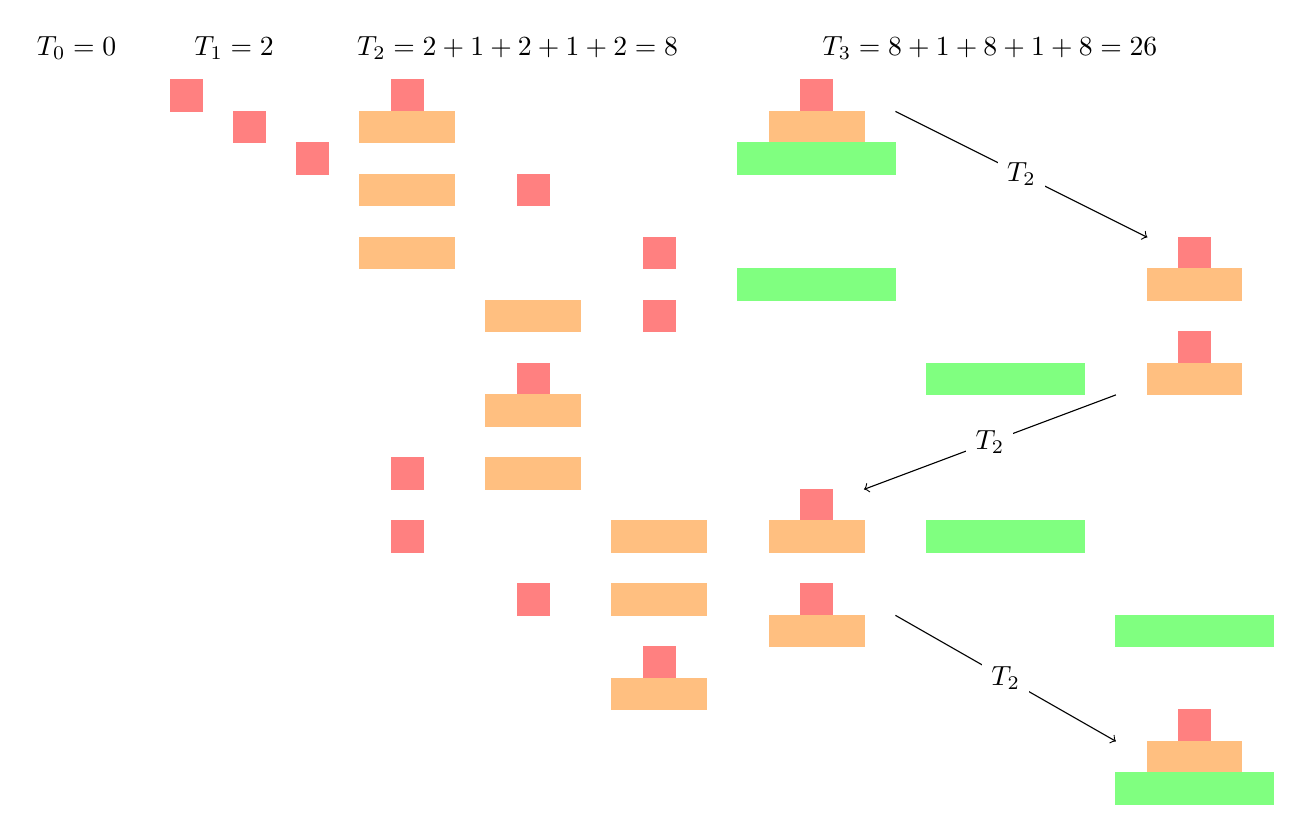
\begin{tikzpicture}[scale=0.8]
\node at (-5,3.5) {$T_0=0$};
\node at (-2.5,3.5) {$T_1=2$};
\filldraw[red!50]  (-3.5,3) rectangle (-3,2.5);
\filldraw[red!50]  (-2.5,2.5) rectangle (-2,2);
\filldraw[red!50]  (-1.5,2) rectangle (-1,1.5);
\node at (2,3.5) {$T_2=2+1+2+1+2=8$};
\filldraw[red!50]  (0,3) rectangle (0.5,2.5);
\filldraw[orange!50]  (-0.5,2.5) rectangle (1,2);
\filldraw[red!50]  (2,1.5) rectangle (2.5,1);
\filldraw[orange!50]  (-0.5,1.5) rectangle (1,1);
\filldraw[red!50]  (4,0.5) rectangle (4.5,0);
\filldraw[orange!50]  (-0.5,0.5) rectangle (1,0);
\filldraw[red!50]  (4,-0.5) rectangle (4.5,-1);
\filldraw[orange!50]  (1.5,-0.5) rectangle (3,-1);
\filldraw[red!50]  (2,-1.5) rectangle (2.5,-2);
\filldraw[orange!50]  (1.5,-2) rectangle (3,-2.5);
\filldraw[red!50]  (0,-3) rectangle (0.5,-3.5);
\filldraw[orange!50]  (1.5,-3) rectangle (3,-3.5);
\filldraw[red!50]  (0,-4) rectangle (0.5,-4.5);
\filldraw[orange!50]  (3.5,-4) rectangle (5,-4.5);
\filldraw[red!50]  (2,-5) rectangle (2.5,-5.5);
\filldraw[orange!50]  (3.5,-5) rectangle (5,-5.5);
\filldraw[red!50]  (4,-6) rectangle (4.5,-6.5);
\filldraw[orange!50]  (3.5,-6.5) rectangle (5,-7);
\node at (9.5,3.5) {$T_3=8+1+8+1+8=26$};
\filldraw[red!50]  (6.5,3) rectangle (7,2.5);
\filldraw[orange!50]  (6,2.5) rectangle (7.5,2);
\filldraw[green!50]  (5.5,2) rectangle (8,1.5);
\filldraw[red!50]  (12.5,0.5) rectangle (13,0);
\filldraw[orange!50]  (12,0) rectangle (13.5,-0.5);
\filldraw[green!50]  (5.5,0) rectangle (8,-0.5);
\filldraw[red!50]  (12.5,-1) rectangle (13,-1.5);
\filldraw[orange!50]  (12,-1.5) rectangle (13.5,-2);
\filldraw[green!50]  (8.5,-1.5) rectangle (11,-2);
\filldraw[red!50]  (6.5,-3.5) rectangle (7,-4);
\filldraw[orange!50]  (6,-4) rectangle (7.5,-4.5);
\filldraw[green!50]  (8.5,-4) rectangle (11,-4.5);
\filldraw[red!50]  (6.5,-5) rectangle (7,-5.5);
\filldraw[orange!50]  (6,-5.5) rectangle (7.5,-6);
\filldraw[green!50]  (11.5,-5.5) rectangle (14,-6);
\filldraw[red!50]  (12.5,-7) rectangle (13,-7.5);
\filldraw[orange!50]  (12,-7.5) rectangle (13.5,-8);
\filldraw[green!50]  (11.5,-8) rectangle (14,-8.5);
\draw (8,2.5) edge[->] node[fill=white] {$T_2$} (12,0.5);
\draw (11.5,-2) edge[->] node[fill=white] {$T_2$} (7.5,-3.5);
\draw (8,-5.5) edge[->] node[fill=white] {$T_2$} (11.5,-7.5);
\end{tikzpicture}

        As we can see, to move the largest one, there should be \textbf{an empty space} on the target peg, because any small disk will be the obstacle of the largest one to put onto the peg. The overall target is to move the largest disk onto the right peg $B$ and process the remaining small pile. The process could be summarized as the following algorithm.

        \begin{codebox}
        \Procname{$\proc{restrictHanoi}(n)$}
        \li \textbf{perform} $\proc{restrictHanoi}(n-1)$.
        \li \textbf{move} the largest disk from the left peg $A$ to the middle peg.
        \li \textbf{reverse} $\proc{restrictHanoi}(n-1)$.
        \li \textbf{move} the largest disk from the middle peg to the right peg $B$.
        \li \textbf{perform} $\proc{restrictHanoi}(n-1)$.
        \end{codebox}

        In other word, denote $T_n$ as the number of the process steps for $n$ disks, the recursive formula could be interpreted as follows:
        
        \begin{equation*}
            T_n = \left\{\begin{aligned}
               &0, && n=0\\
               &T_{n-1}+1+T_{n-1}+1+T_{n-1}, && n>0\\
            \end{aligned}\right.
        \end{equation*}

        The formula could be simplified as the following process:
        \begin{align*}
            T_n &= 3T_{n-1} + 2 \\
            T_n + 1 &= 3(T_{n-1}+1) \\
            T_n + 1 &= 3^n \\
            T_n &= 3^n -1 
        \end{align*}


    \end{solution}

    \item[3] Show that, in the process of transferring a tower under the restrictions of the preceding exercise, we will actually encounter every properly stacked arrangement of $n$ disks on three pegs.
    
    \begin{proof}
        \begin{lemma}\label{lem:count}
            There are $3^n$ arrangements for $n$ disks.
        \end{lemma}

        Because every disk has three options to lay and once the peg has multiple disks, the arrangement is fixed as the bigger disk always at a lower layer.

        \begin{lemma}\label{lem:unique}
            The states are unique.
        \end{lemma}

        Because the procedure is required to be the \textbf{shortest}. Any identical states could be skipped in order to obtain a shorter process.

        By combining Lemma \ref{lem:count} and Lemma \ref{lem:unique}, the shortest $3^n-1$ steps corresponde to $3^n$ unqiue states. So every properly stacked arrangement of $n$ disks on three pegs is encountered.
    \end{proof}

    \item[4] Are there any starting and ending configurations of $n$ disks on three pegs that are more than $2^n-1$ moves apart, under Lucas's original rules?
    
    \begin{solution}
        \textbf{No more moves are required. Use the mathematical induction.} When $n=0$, no move is needed. When $n=1$, only $1=2^1-1$ move is needed to move the disk from any peg to the other.
        
        If $2^{k-1}-1$ is sufficient for any starting and ending configurations with $n-1$ disks, then 
        \begin{description}
            \item[Case 1] \textbf{The largest disk is on the same peg for the starting and ending configurations.} By induction, $2^{k-1}-1$ is enough for moving $n-1$ disks.
            \item[Case 2] \textbf{The largest disk changes its position between the starting and ending configurations.} 
            
            \begin{enumerate}
                \item Move $n-1$ disks and change the case into the middle configuration where there is an empty for the target peg where the largest disk lands.
                \item Move the largest peg onto the target end peg.
                \item Move $n-1$ disks from the previous state to the ending configuration.
            \end{enumerate}

            As a result, it requires $2^{k-1}-1+1+2^{k-1}-1=2^k-1$ moves.
        \end{description}
        The $2^k-1$ is sufficient for $k$ disks. By the principle of mathematical induction, there is no starting and ending configurations of $n$ disks that requires $2^n-1$ moves.
    \end{solution}
    
    \item[5] A ``Venn diagram'' with three overlapping circles is often used to illustrate the eight possible subsets associated with three given sets:
    
    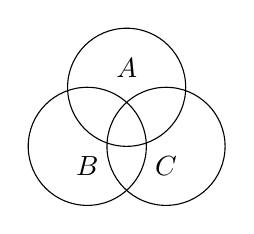
\begin{tikzpicture}[scale=0.5]
\draw  (-2,3.5) node[above] {$A$}  ellipse (1.5 and 1.5);
\draw  (-3,2) node[below] {$B$} ellipse (1.5 and 1.5);
\draw  (-1,2) node[below] {$C$} ellipse (1.5 and 1.5);
\end{tikzpicture}


    Can the sixteen possibilities that arise with four given sets be illustrated by four overlapping circles?

    \begin{solution}
        \textbf{It is impossible.} To construct the fourth circle based on the original three circles, the edge of the new circle must divide every original possible into halfs.

        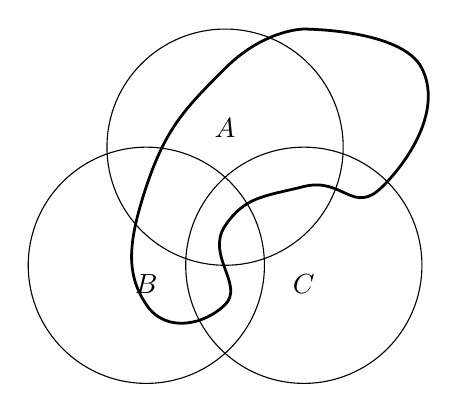
\begin{tikzpicture}
\draw  (-2,3.5) node[above] {$A$}  ellipse (1.5 and 1.5);
\draw  (-3,2) node[below] {$B$} ellipse (1.5 and 1.5);
\draw  (-1,2) node[below] {$C$} ellipse (1.5 and 1.5);
\draw[line width=1pt]  plot[smooth, tension=.9] coordinates {(-1,5) (-2,4.5) (-3,3) (-3,1.5) (-2,1.5) (-2,2.5) (-1,3) (0,3) (0.5,4.5) (-1,5)};
\end{tikzpicture}


        This will make the new edge must get four intersections with one of the circle ($A$ in this case). But two circles only get at most two intersections. So it is impossible.
    \end{solution}

\end{problems}

\end{document}
